\section{Hardware Implementation}

The CLAS12 Trigger System is implemented using High Speed Serial (VXS) techniques for a complete fully pipelined multi-crate Trigger System that takes advantage of the elegant high-speed VXS serial extensions for VME.  This Trigger System includes a pre-trigger level and three stages, starting with the front-end VXS crate Trigger Processor (VTP), a sector-level SubSystem Processor (SSP), a global VTP processor (GTP), and a Trigger Supervisor (TS) that manages the timing, synchronization, and front-end event readout.

Within a front-end crate, the trigger information is gathered from the pre-trigger boards, consisting of 16-channel, 12-bit FADC and 96-channel DCRB (\cite{daq-ref}) modules via the VXS backplane, to a VXS Trigger Processor (VTP). Each VTP is capable of handling these 500~MBps VXS links from the 16 modules, and then performs real-time crate-level trigger algorithms.  The VTP transmits the Stage 1 trigger information through multiple Gigabit transceivers that are combined into a fiber link. The VTP uses a multi-fiber link to increase the aggregate trigger data transfer rate to the global trigger to 10~Gbps.

The trigger data is transmitted on the VXS backplane, and on the multi-fiber link using the Aurora protocol from Xilinx.  The front-end VXS modules use Virtex-V devices with Gigabit Transceivers operating at 2.5~Gbps. The VTP collects these serial streams with a Virtex-7 device and works with a Zynq7 processor to manage the network interface and on-board Linux operating system.

The entire Trigger System is synchronous and operates at 250~MHz with the Trigger Supervisor managing not only the front-end event readout, but also the distribution of the critical timing clocks, synchronization signals, and the global trigger signals to each front-end readout crate.  These signals are distributed to the front-end crates on a separate fiber link, and each crate is synchronized using a unique encoding scheme to guarantee that each front-end crate is synchronous with a fixed latency, independent of the distance between each crate.  The overall trigger signal latency is $<$8~$\mu$s, and the CLAS12 experiments require a trigger rate of up to 20~kHz, which can be easily handled since the hardware has an ability to operate with a trigger rate of up to 200~kHz. The following sections describe the main Trigger System hardware components.


\subsection{Pre-trigger Boards}

Two type of boards are used at the pre-trigger level to supply information to the trigger system: FADC and DCRB. They are described in detail in the CLAS12 DAQ paper \cite{daq-ref}.

\subsection{VTP Board}
\label{sec:vtp_board}

\begin{figure}[hbt]
	\centering
	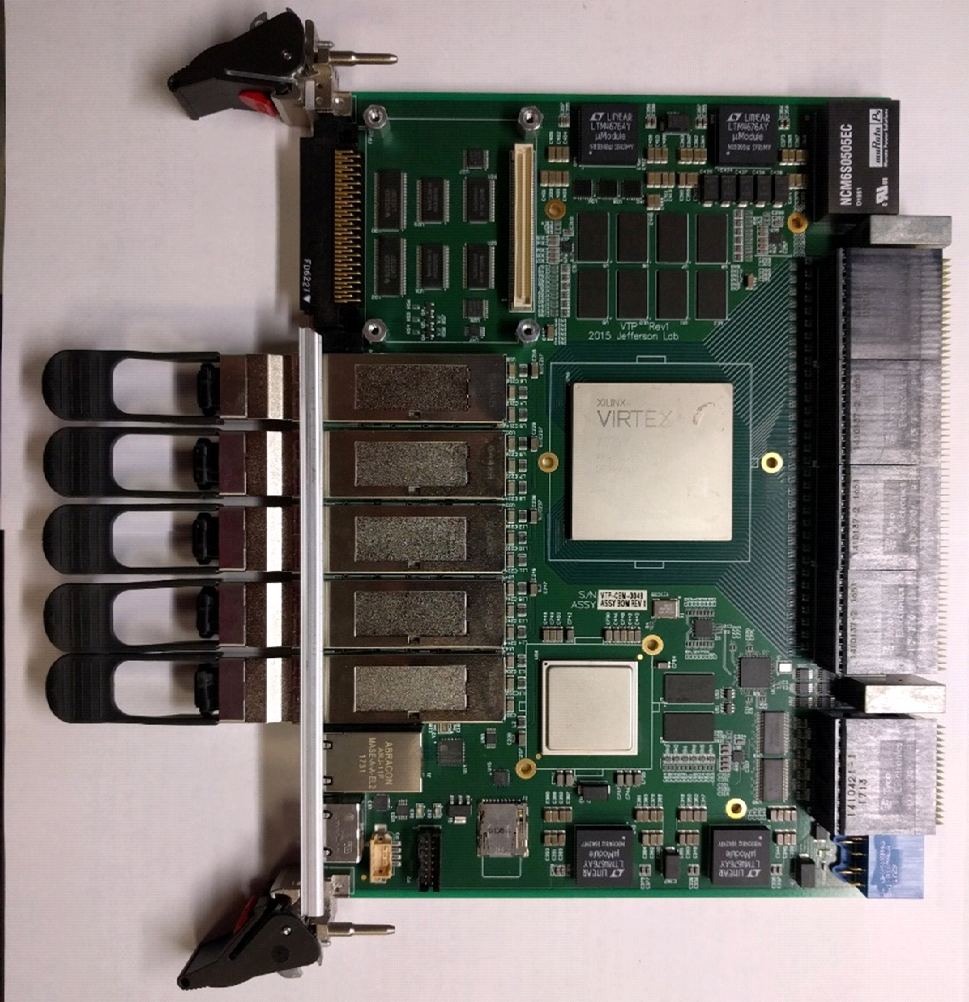
\includegraphics[width=1.0\columnwidth,keepaspectratio]{img/vtp_board.png}
	\caption{VXS Trigger Processor (VTP) Board. Based on Xilinx XC7V550T FPGA, the board is the processing unit of the Stage 1 and Stage 3 Trigger System. In addition to making the trigger decision, it also reports the corresponding information into the data stream for debugging purposes.}
	\label{fig:vtp_board}
\end{figure}

The VXS Trigger Processor (VTP, see Fig.~\ref{fig:vtp_board}) is a VXS switch card that is used to implement trigger logic on the front-end crates (Stage 1) and global trigger crate (Stage 3). There are 80 full-duplex serial links each capable of running at up to 8.5~Gbps that can be used for transporting the trigger data. The links are bonded in groups of 4 for a total of 20 channels, which include 16 VXS payload slot interfaces (copper) and 4 QSFP interfaces (optical).

\paragraph{Front-end (Stage 1) Crate Processing}
The VTP in the front-end crate collects data from the VXS payload FADC and DCRB modules (and optionally from some of the QSFP links), where it aligns the data in time for all links, and presents it to the detector-specific trigger logic, which resides in a XC7V550T FPGA. The trigger logic processes the data and produces an output trigger stream that is sent to the Stage 2 trigger crate (and optionally to other Stage 1 VTP modules) using up to 4 QSFP optical links. The QSFP optical links allow the Stage 1 trigger logic to use information from multiple Stage 1 crates, which is required for some detectors that span multiple VXS crates (e.g. the DC and FT subsystems). The QSFP optical links also allow multiple links to go to Stage 2 when more bandwidth is needed (e.g. HTCC and CTOF).

\paragraph{Global Trigger (Stage 3) Crate Processing}
In the global trigger crate the VTP collects data from the VXS payload SSP modules. The SSP modules supply a stream of trigger bits for each sector (HTCC, FTOF, EC, PCAL, and DC) and also a stream of trigger bits for the central detectors (CTOF, CND, and FT). These sector and central trigger bit streams have already performed timing, multiplicity, and geometry coincidences between the detectors within the sector or central detectors. The Stage 3 VTP allows the final (``global'') trigger bits (up to 32) to be defined using different combinations for sectors, sector trigger bits, and central trigger bits. The 32 global trigger bit decisions are evaluated at 250~MHz so that no additional jitter is introduced by this stage. These bits are sent to the TS using the high-density LVDS front-panel output using a twisted-pair ribbon cable.

\paragraph{Event Builder}
A Zynq FPGA is used on the VTP to run the standard CLAS12 CODA readout controller (ROC) component, which allows the VTP to be configured and read out the same as other VME/Intel-based CODA components. Event data can be generated by the VTPs that contain the trigger decisions for both the Stage 1 and 3 components, which is used to understand the trigger efficiency. Additionally, there is a large buffer (4~GB with 200~Gbps bandwidth) and 40~Gbps Ethernet interface that is intended for future upgrades of the front-end crate readout system, which would use the VTP and 40~Gbps Ethernet for event readout rather than the VME interface. Fig.~\ref{fig:vtp_block_daq} shows the interfaces between the FPGAs, memory, network, VXS, and fiber modules.

\begin{figure}[hbt]
	\centering
	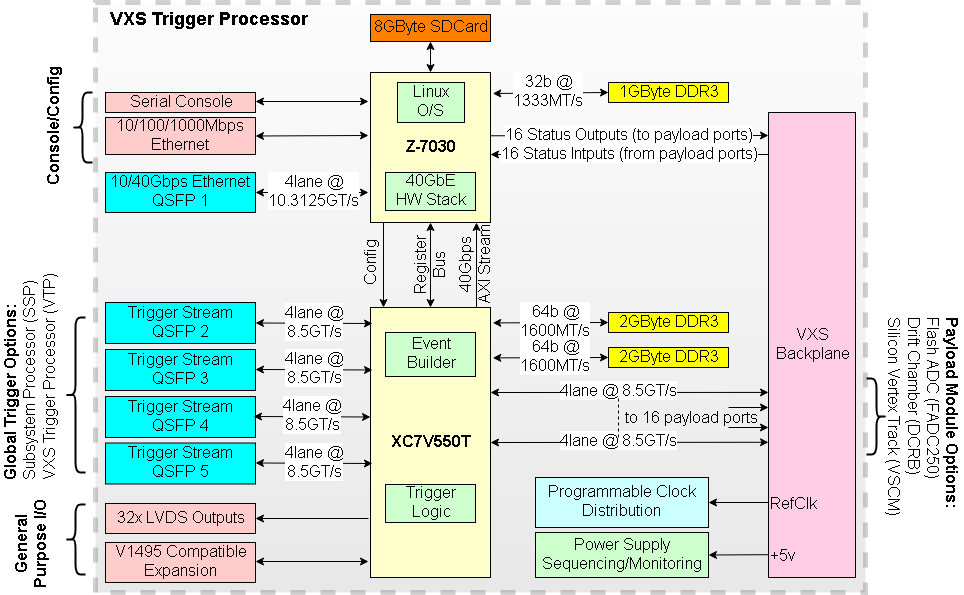
\includegraphics[width=1.0\columnwidth,keepaspectratio]{img/vtp_block_daq.png}
	\caption{VXS Trigger Processor Board (VTP) Block Diagram. This module is a single board computer designed in JLab to execute the most resource-consuming algorithms of the trigger logic.}
	\label{fig:vtp_block_daq}
\end{figure}


\subsection{SSP Board}
\label{sec:ssp_board}

\begin{figure}[hbt]
	\centering
	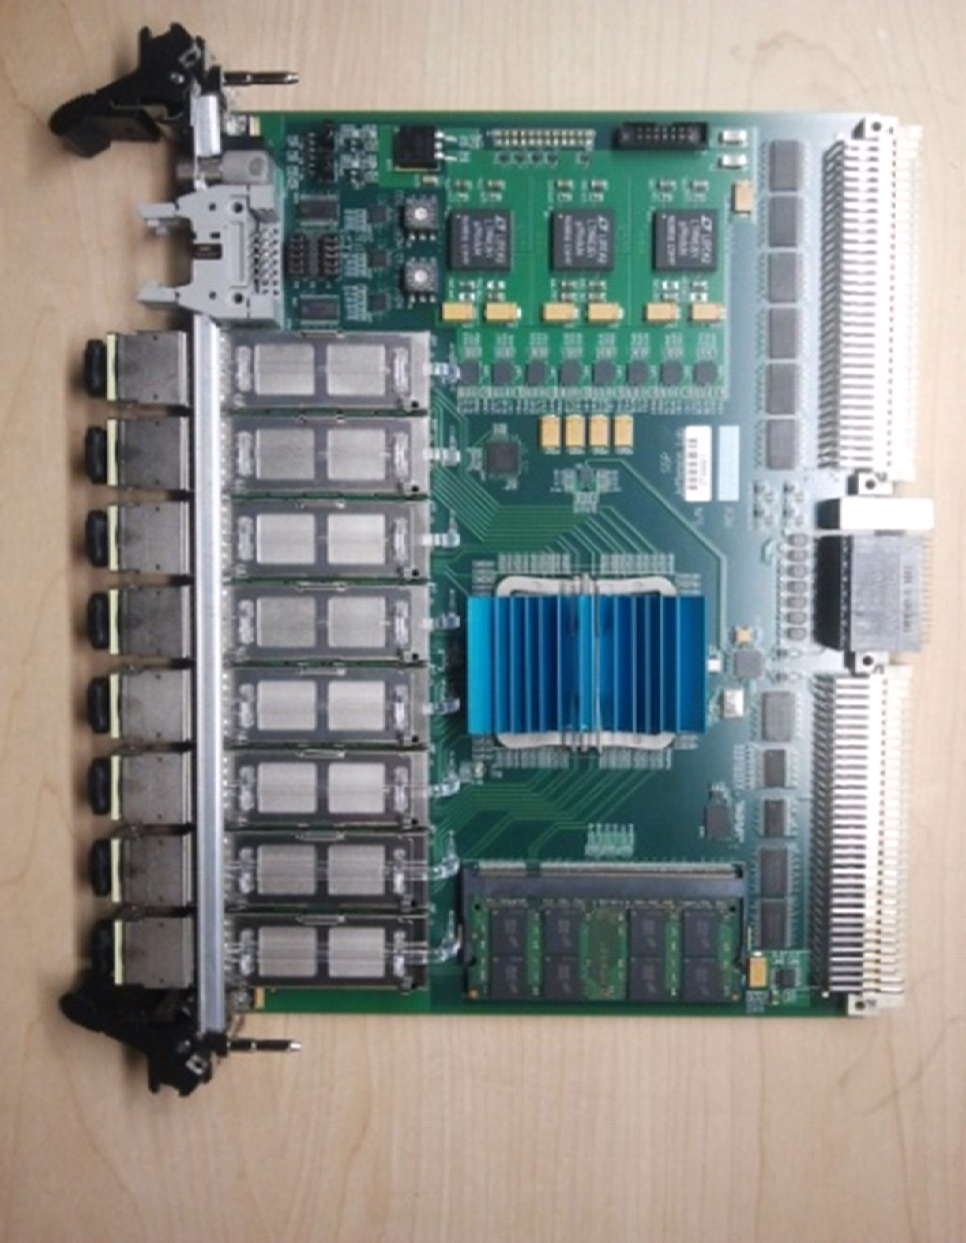
\includegraphics[width=1.0\columnwidth,keepaspectratio]{img/ssp_board.png}
	\caption{SubSystem Processor (SSP) Board. Based on a Xilinx XC5VTX150T FPGA, it is responsible for the making the Stage 2 trigger decision.}
	\label{fig:ssp_board}
\end{figure}

The SubSystem Processor (SSP, see Fig.~\ref{fig:ssp_board}) is a VXS payload card used to collect data from multiple front-end (Stage 1) crates. The SSP performs the Stage 2 trigger processing by creating sector and central trigger bit decisions. Up to 16 SSP modules can be housed in a single VXS crate, but only 7 are currently needed: 6 for the sector-based detectors and 1 for the central detectors. There are 36 full-duplex serial links each capable of running at up to 6.5~Gbps that can be used for transporting the trigger data. The links are bonded in groups of 4 for a total of 8 channels: 1 VXS switch slot interface (copper) and 8 QSFP interfaces (optical). All VXS and QSFP lanes run at 5~Gbps (or 20~Gbps per channel).

\paragraph{Stage 2 Trigger Processing}
The Stage 1 optical data arrives at the SSP where it is aligned and processed through various algorithms to make the sector and central trigger bit decisions. There are 8 sector and central trigger bits (expandable to 32) that evaluate at 250~MHz so that no jitter is introduced by this stage. These bits are sent to the Stage 3 VTP using the VXS switch serial interface. As for the VTP, the SSP has an Event Builder that allows for readout of the trigger information and its insertion into the data stream.
